% TODO:
% 1) 













%%%%%%%%%%%%%%%%%%%%%%%%%%%%%%%%%%%%%%%%%
% Beamer Presentation
% LaTeX Template
% Version 1.0 (10/11/12)
%
% This template has been downloaded from:
% http://www.LaTeXTemplates.com
%
% License:
% CC BY-NC-SA 3.0 (http://creativecommons.org/licenses/by-nc-sa/3.0/)
%
%%%%%%%%%%%%%%%%%%%%%%%%%%%%%%%%%%%%%%%%%

%----------------------------------------------------------------------------------------
%	PACKAGES AND THEMES
%----------------------------------------------------------------------------------------

\documentclass{beamer}

\mode<presentation> {

% The Beamer class comes with a number of default slide themes
% which change the colors and layouts of slides. Below this is a list
% of all the themes, uncomment each in turn to see what they look like.

%\usetheme{default}
%\usetheme{AnnArbor}
%\usetheme{Antibes}
%\usetheme{Bergen}
%\usetheme{Berkeley}
%\usetheme{Berlin}
%\usetheme{Boadilla}
%\usetheme{CambridgeUS}
%\usetheme{Copenhagen}
%\usetheme{Darmstadt}
%\usetheme{Dresden}
%\usetheme{Frankfurt}
%\usetheme{Goettingen}
%\usetheme{Hannover}
%\usetheme{Ilmenau}
%\usetheme{JuanLesPins}
%\usetheme{Luebeck}
\usetheme{Madrid}
%\usetheme{Malmoe}
%\usetheme{Marburg}
%\usetheme{Montpellier}
%\usetheme{PaloAlto}
%\usetheme{Pittsburgh}
%\usetheme{Rochester}
%\usetheme{Singapore}
%\usetheme{Szeged}
%\usetheme{Warsaw}

% As well as themes, the Beamer class has a number of color themes
% for any slide theme. Uncomment each of these in turn to see how it
% changes the colors of your current slide theme.

%\usecolortheme{albatross}
%\usecolortheme{beaver}
%\usecolortheme{beetle}
%\usecolortheme{crane}
%\usecolortheme{dolphin}
%\usecolortheme{dove}
%\usecolortheme{fly}
%\usecolortheme{lily}
%\usecolortheme{orchid}
%\usecolortheme{rose}
%\usecolortheme{seagull}
%\usecolortheme{seahorse}
%\usecolortheme{whale}
%\usecolortheme{wolverine}

%\setbeamertemplate{footline} % To remove the footer line in all slides uncomment this line
%\setbeamertemplate{footline}[page number] % To replace the footer line in all slides with a simple slide count uncomment this line

%\setbeamertemplate{navigation symbols}{} % To remove the navigation symbols from the bottom of all slides uncomment this line
}

\usepackage[utf8]{inputenc}
\usepackage[russian]{babel}
\usepackage{cmap}


\usepackage{verbatim}
\usepackage{fancybox}
\usepackage{ulem}
\usepackage{tikz}
\usetikzlibrary{positioning}
\usepackage{scalefnt}
\usetikzlibrary{arrows,shapes,positioning,shadows,trees,calc,backgrounds,fit,positioning}

\usepackage{graphicx} % Allows including images
\usepackage{booktabs} % Allows the use of \toprule, \midrule and \bottomrule in tables
\usepackage{textcomp}
\usepackage{listings}
\usepackage{color}
\usepackage{xcolor}
\usepackage{changepage}

\definecolor{mygreen}{rgb}{0,0.6,0}
\definecolor{mygray}{rgb}{0.5,0.5,0.5}
\definecolor{mymauve}{rgb}{0.58,0,0.82}

\lstset{ %
  backgroundcolor=\color{white},   % choose the background color; you must add \usepackage{color} or \usepackage{xcolor}
  basicstyle=\footnotesize,        % the size of the fonts that are used for the code
  breakatwhitespace=false,         % sets if automatic breaks should only happen at whitespace
  breaklines=true,                 % sets automatic line breaking
  captionpos=b,                    % sets the caption-position to bottom
  commentstyle=\color{mygreen},    % comment style
  deletekeywords={...},            % if you want to delete keywords from the given language
  escapeinside={\%*}{*)},          % if you want to add LaTeX within your code
  extendedchars=true,              % lets you use non-ASCII characters; for 8-bits encodings only, does not work with UTF-8
  frame=single,                    % adds a frame around the code
  keepspaces=true,                 % keeps spaces in text, useful for keeping indentation of code (possibly needs columns=flexible)
  keywordstyle=\color{blue},       % keyword style
  language=Octave,                 % the language of the code
  morekeywords={*,...},            % if you want to add more keywords to the set
  numbers=left,                    % where to put the line-numbers; possible values are (none, left, right)
  numbersep=5pt,                   % how far the line-numbers are from the code
  numberstyle=\tiny\color{mygray}, % the style that is used for the line-numbers
  rulecolor=\color{black},         % if not set, the frame-color may be changed on line-breaks within not-black text (e.g. comments (green here))
  showspaces=false,                % show spaces everywhere adding particular underscores; it overrides 'showstringspaces'
  showstringspaces=false,          % underline spaces within strings only
  showtabs=true,                  % show tabs within strings adding particular underscores
  stepnumber=1,                    % the step between two line-numbers. If it's 1, each line will be numbered
  stringstyle=\color{mymauve},     % string literal style
  tabsize=4,                       % sets default tabsize to 2 spaces
  %title=\lstname                   % show the filename of files included with \lstinputlisting; also try caption instead of title
}

\graphicspath{{./figures/}}

%----------------------------------------------------------------------------------------
%	TITLE PAGE
%----------------------------------------------------------------------------------------

\title[Обработка и исполнение запросов: лекция 8]{Обработка и исполнение запросов в СУБД (Лекция 8) \\~\\ Колоночные СУБД в оперативной памяти\\~\\ v6} % The short title appears at the bottom of every slide, the full title is only on the title page

\author{Георгий Чернышев} % Your name
\institute[ВШЭ] % Your institution as it will appear on the bottom of every slide, may be shorthand to save space
{
Высшая Школа Экономики \\ % Your institution for the title page
\medskip
\textit{chernishev@gmail.com} % Your email address
}
%\date{\today} % Date, can be changed to a custom date
\date{21 октября 2020 г.}
\begin{document}

\begin{frame}
\titlepage % Print the title page as the first slide
\end{frame}

\begin{comment}
\begin{frame}
\frametitle{Overview} % Table of contents slide, comment this block out to remove it
\tableofcontents % Throughout your presentation, if you choose to use \section{} and \subsection{} commands, these will automatically be printed on this slide as an overview of your presentation
\end{frame}


\begin{frame}
\frametitle{Долг: данные на диске}

В двух словах (очень приблизительно):

\begin{itemize}
  \setlength\itemsep{1em}
  \item Данных хранятся на диске;
  \item Считываются и \alert{временно} хранятся в памяти;
  \item Обычно какой-то memory mapping;
  \item Менджер буферов (buffer-manager): считывание, удержание в памяти, модификация данных, сброс на диск;
  \begin{itemize}
    \item pin/unpin;
    \item алгоритм замещения: LRU, Clock algorithm, MRU, ...
  \end{itemize}
  \item ``Нарезка'' на страницы: единицы оперирования менеджера буферов, 4-8 KB;
\end{itemize}

Кому интересно дальше: \small{\url{https://web.stanford.edu/class/cs346/2015/notes/Lecture_One.pdf}}

Как представлять страницу? Записи ведь бывают переменной длины!

\end{frame}

\begin{frame}
\frametitle{Долг: слотированная страница}

\begin{figure}[htb]
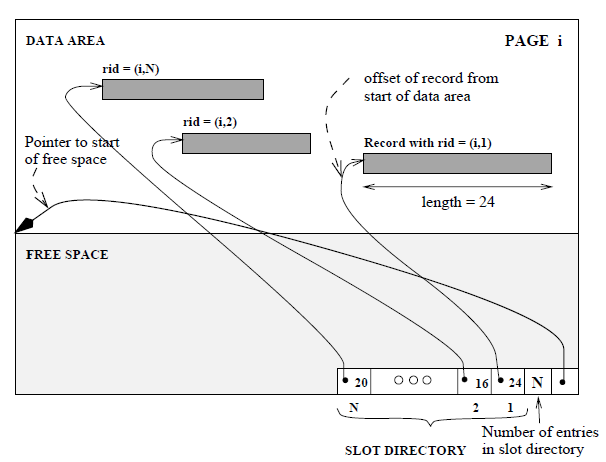
\includegraphics[width=\textwidth,height=0.8\textheight,keepaspectratio]{slotted.png} 
\footnote{\tiny{Изображение взято из \cite{Ramakrishnan2000}}}
\end{figure}

\end{frame}
\end{comment}

\begin{frame}
\frametitle{План}

Рассмотрим систему MonetDB~--- колоночную систему в оперативной памяти.

\begin{itemize}
	\setlength\itemsep{1em}
	\item MonetDB, ее принципы устройства, планы запросов
	\item Аппаратные основания для появления MonetDB
	\item MonetDB как исследовательская платформа:
	\begin{itemize}
		\setlength\itemsep{1em}
		\item Cache-conscious соединение
		\item Database cracking
		\item Recycler
	\end{itemize}
	\item Буфер-менеджер "на пальцах"
	\item MonetDB/X100

\end{itemize}
\end{frame}

\begin{frame}
\frametitle{MonetDB~--- колоночная СУБД в памяти}

Вкратце из статей, например \cite{Boncz1999, Boncz2008}:

\begin{itemize}
	%\setlength\itemsep{1em}
	\item Данные представлены в виде BAT структур (Binary Association Table): набор пар $(key, value)$;
	\item Над BAT есть своя алгебра: каждый оператор работает над одним или несколькими BAT, возвращает BAT;
	\item Не Volcano, а operator-at-a-time model;
	\item Каждый оператор очень простой. Фактически, реализация операций над массивом;
	\item Все данные в памяти, mmap-ом отображаются на диск, если виртуальной памяти не хватит, используем за-mmap-леную дисковую, есть подсистема (это вместо буфер-менеджера).	
\end{itemize}

Этот подход позволяет очень эффективно использовать процессор и оперативную память.

\end{frame}

\begin{frame}
\frametitle{Простой пример}

\begin{figure}[htb]
	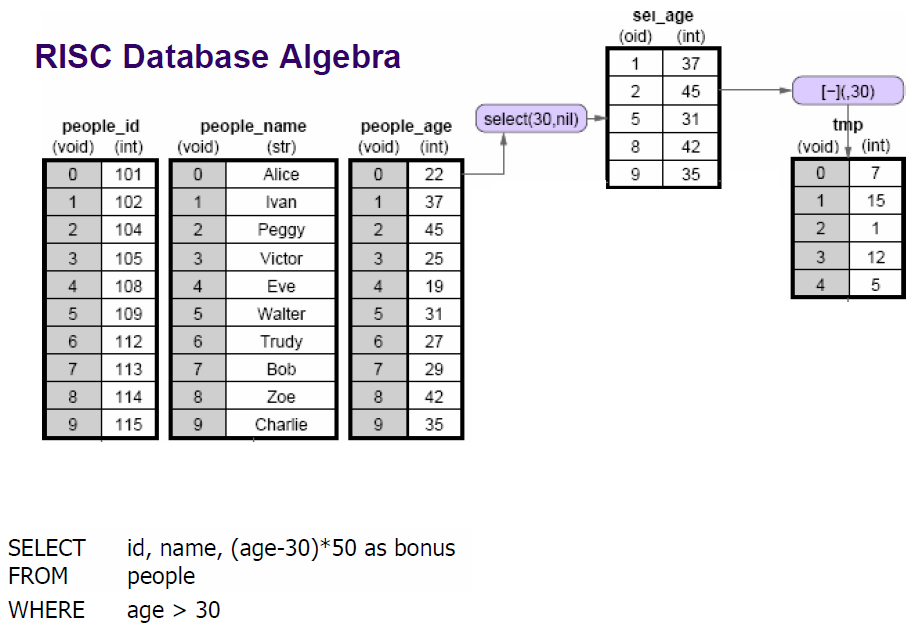
\includegraphics[width=\textwidth,height=0.750\textheight,keepaspectratio]{example.png} 
	\footnote{\tiny{Изображение взято из \cite{Harizopoulos2009}}}
\end{figure}    

\end{frame}

\begin{frame}
\frametitle{Пример посложнее (смотрите в план в pdf)}

\begin{figure}[htb]
	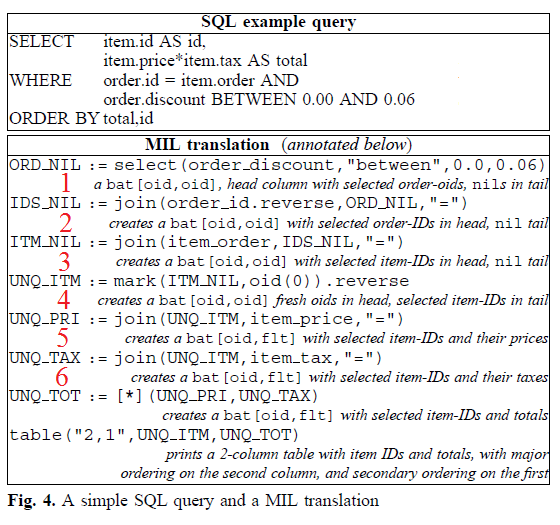
\includegraphics[width=\textwidth,height=0.750\textheight,keepaspectratio]{example2.png} 
	\footnote{\tiny{Изображение взято из \cite{Boncz1999}}}
\end{figure}    

\end{frame}



\begin{frame}
\frametitle{Про ``железо'' ``на пальцах'' I}

\begin{figure}[htb]
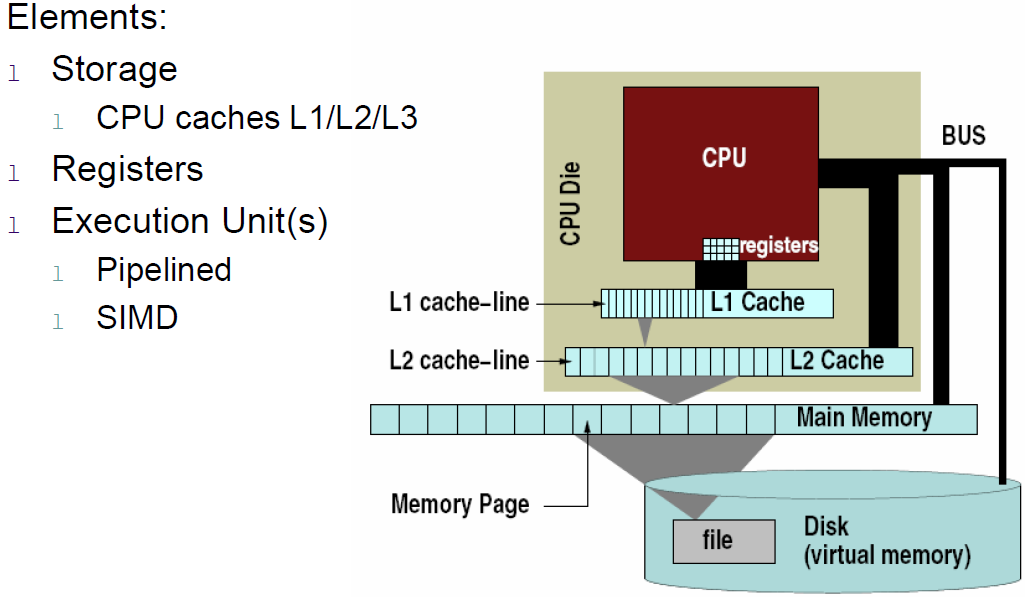
\includegraphics[width=\textwidth,height=0.750\textheight,keepaspectratio]{processor.png} 
\footnote{\tiny{Изображение взято из \cite{Harizopoulos2009}}}
\end{figure}    
  
\end{frame}

\begin{frame}
\frametitle{Про ``железо'' ``на пальцах'' II (SIMD)}

\begin{figure}[htb]
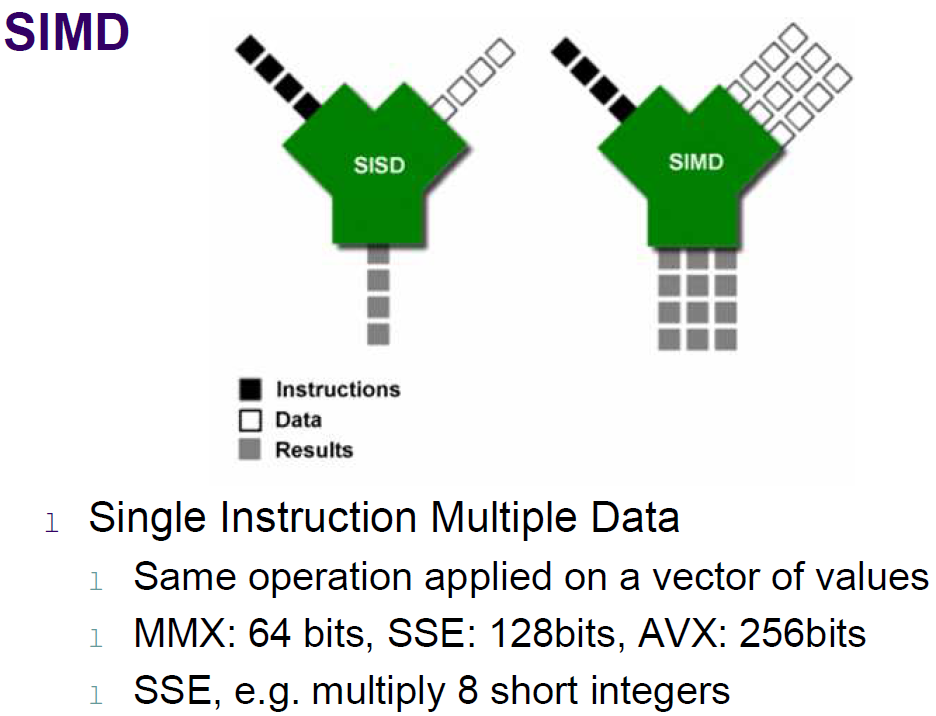
\includegraphics[width=\textwidth,height=0.750\textheight,keepaspectratio]{simd.png} 
\footnote{\tiny{Изображение взято из \cite{Harizopoulos2009}}}
\end{figure}    
  
\end{frame}


\begin{frame}
\frametitle{Про ``железо'' ``на пальцах'' III (эволюция процессоров)}

\begin{figure}[htb]
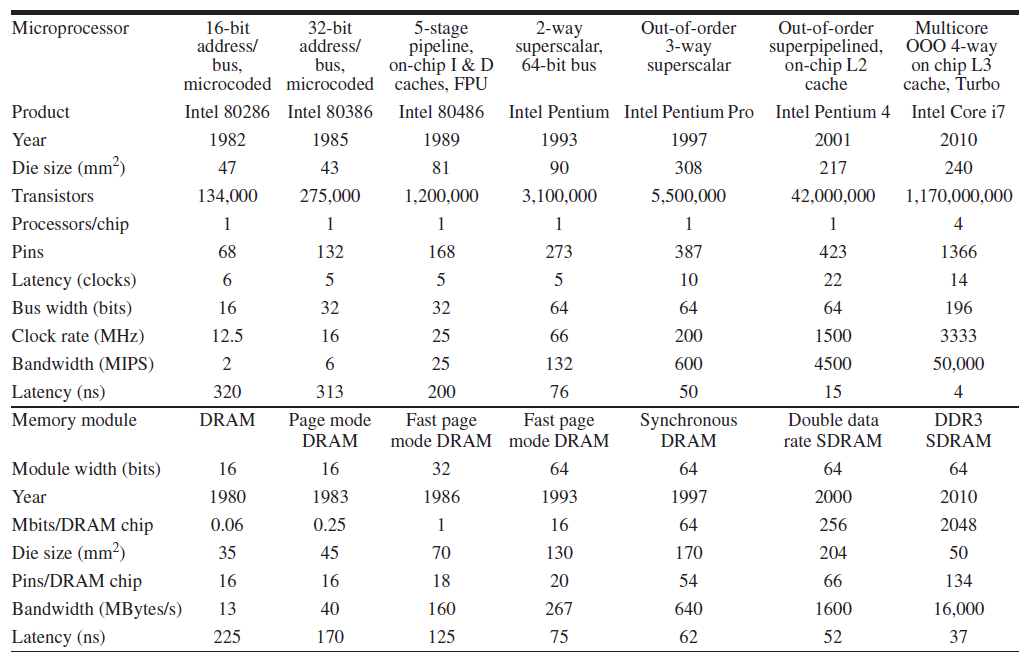
\includegraphics[width=\textwidth,height=0.750\textheight,keepaspectratio]{stats2.png} 
\footnote{\tiny{Изображение взято из \cite{Hennessy2011}}}
\end{figure}    
  
\end{frame}

\begin{frame}
\frametitle{Про ``железо'' ``на пальцах'' IV (25 лет эволюции RAM)}

\begin{figure}[htb]
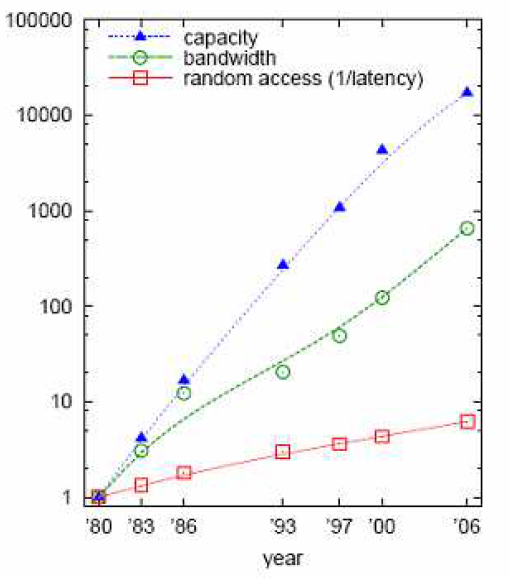
\includegraphics[width=\textwidth,height=0.80\textheight,keepaspectratio]{dram.png} 
\footnote{\tiny{Изображение взято из \cite{Harizopoulos2009}}}
\end{figure}    
  
\end{frame}

\begin{frame}
\frametitle{Про ``железо'' ``на пальцах'' V (иерархия носителей)}

\begin{figure}[htb]
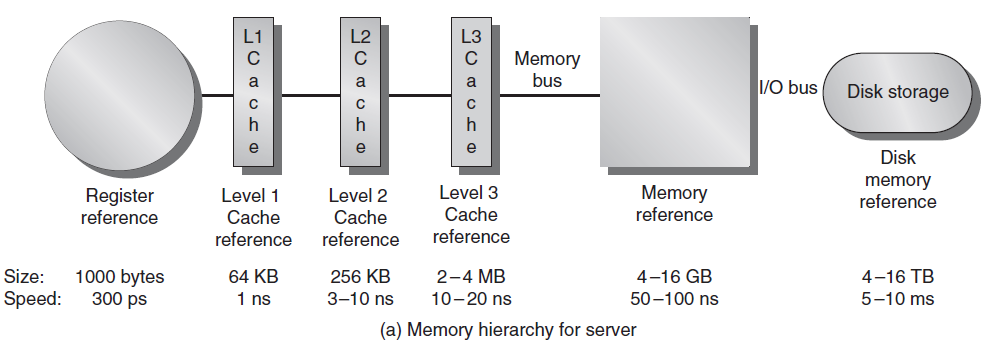
\includegraphics[width=\textwidth,height=0.750\textheight,keepaspectratio]{memoryhierarchy2.png} 
\footnote{\tiny{Изображение взято из \cite{Hennessy2011}}}
\end{figure}    
  
\end{frame}

\begin{frame}
\frametitle{Про ``железо'' ``на пальцах'' VI (стоимость операций)}

\begin{figure}[htb]
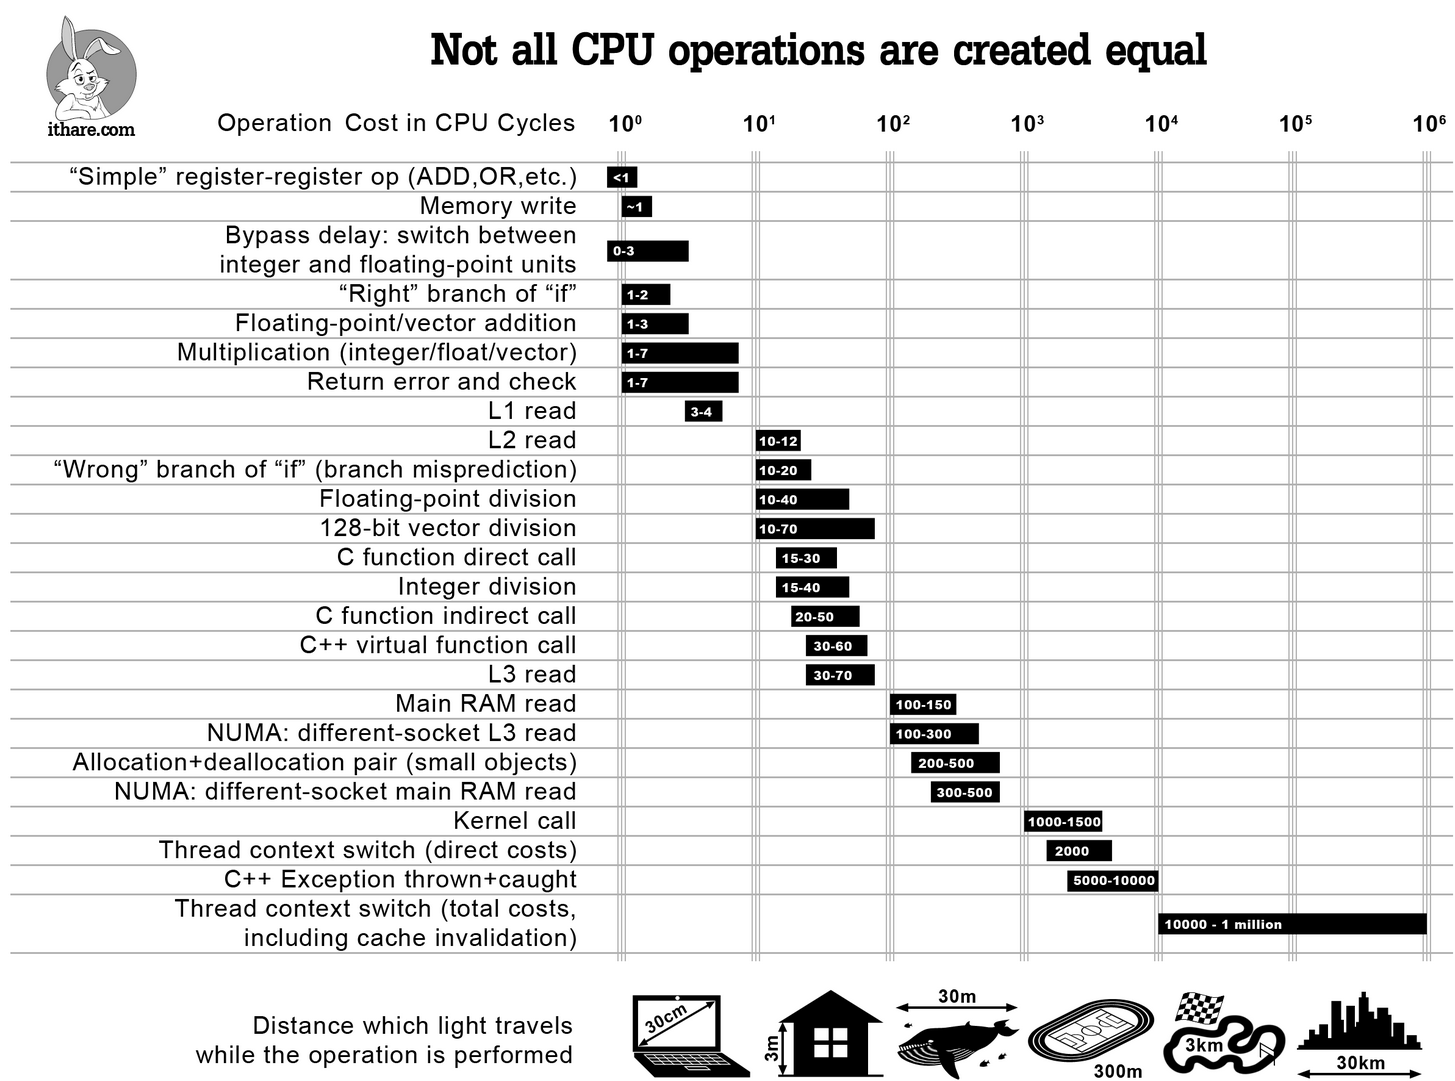
\includegraphics[width=\textwidth,height=0.750\textheight,keepaspectratio]{times.png} 
\footnote{\tiny{Изображение взято из \url{http://ithare.com/wp-content/uploads/part101_infographics_v07.png}}}
\end{figure}    
  
\end{frame}

\begin{frame}
\frametitle{О кеш-памяти}

Бывает:
\begin{itemize}
  \item Кеш данных~--- хранит данные, которыми оперирует программа,
  \item Кеш инструкций~--- хранит саму программу.
\end{itemize}

\begin{figure}[htb]
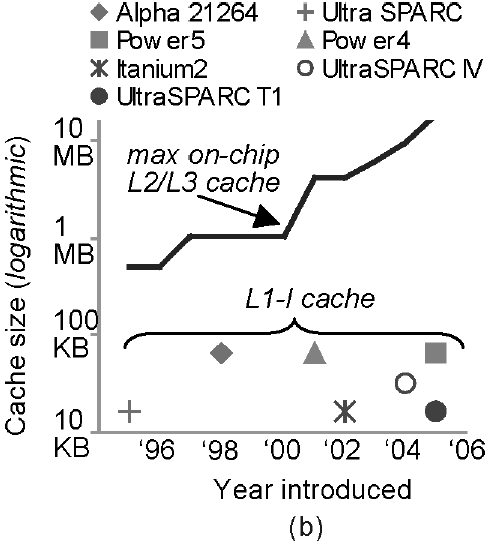
\includegraphics[width=\textwidth,height=0.63\textheight,keepaspectratio]{cache1.png} 
\footnote{\tiny{Изображение взято из \cite{Harizopoulos2006}}}
\end{figure}   

\end{frame}

\begin{frame}
\frametitle{Как выглядит код в кеш-памяти}

\begin{figure}[htb]
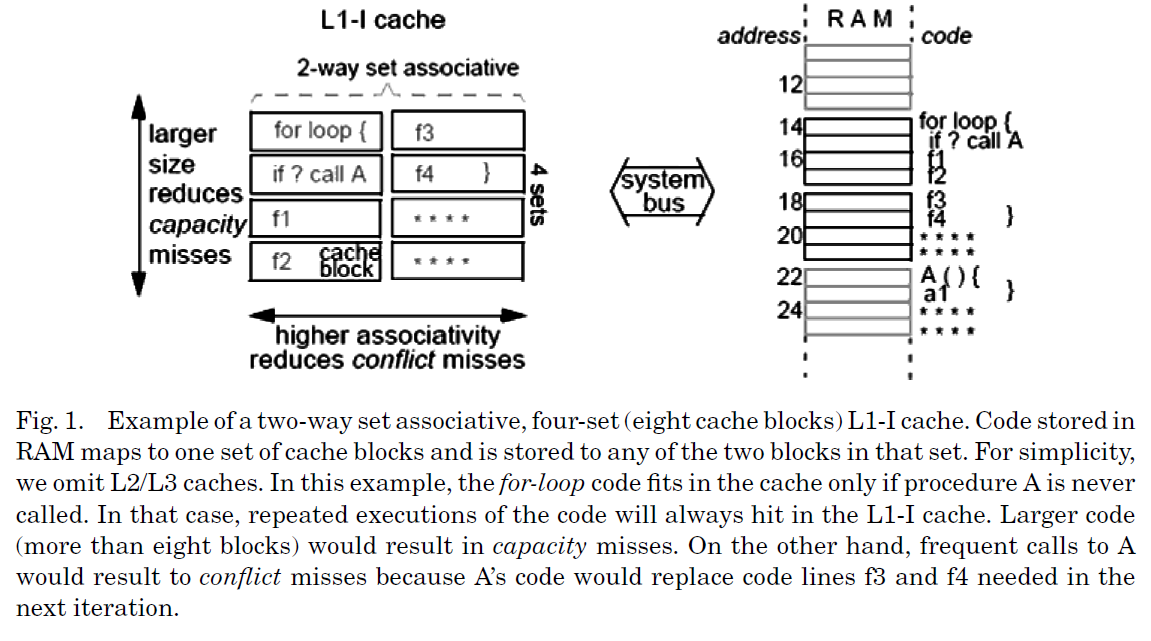
\includegraphics[width=\textwidth,height=0.73\textheight,keepaspectratio]{cache2.png} 
\footnote{\tiny{Изображение взято из \cite{Harizopoulos2006}}}
\end{figure}   

\end{frame}

\begin{frame}
\frametitle{Кеш-память и цифры}

\begin{itemize}
  \setlength\itemsep{1em}
  \item L1 кеш 8-64KB (и данные, и инструкции), больше не будет:
  \begin{itemize}
    \item придется снижать частоту, температура
  \end{itemize}
  \item В OLTP код занимает 556 KB, смотри ссылку из \cite{Harizopoulos2006}.
\end{itemize}

То есть, для достижения хорошей производительности надо писать ``правильный'' код.

\end{frame}

\begin{frame}
\frametitle{Про ``железо'' ``на пальцах'' VII: конвейер}

\begin{figure}[htb]
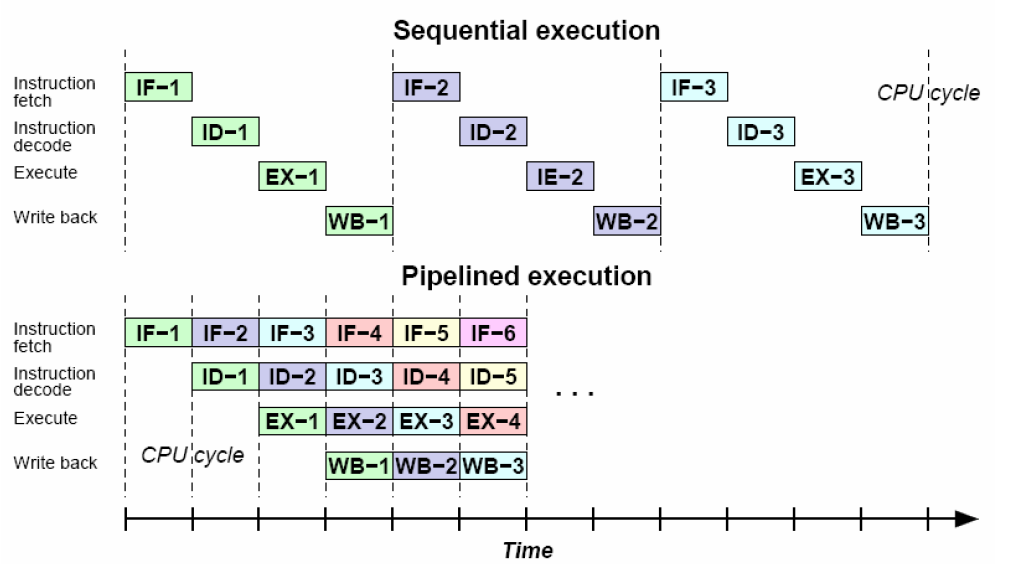
\includegraphics[width=\textwidth,height=0.680\textheight,keepaspectratio]{superscalar.png} 
\footnote{\tiny{Изображение взято из \cite{Harizopoulos2009}}}
\end{figure}
{
\scriptsize
Кому непонятно, читайте \url{https://en.wikipedia.org/wiki/Instruction_pipelining}.
}
\end{frame}



\begin{frame}
\frametitle{Про ``железо'' ``на пальцах'' VIII: проблемы выполнения}

\begin{figure}[htb]
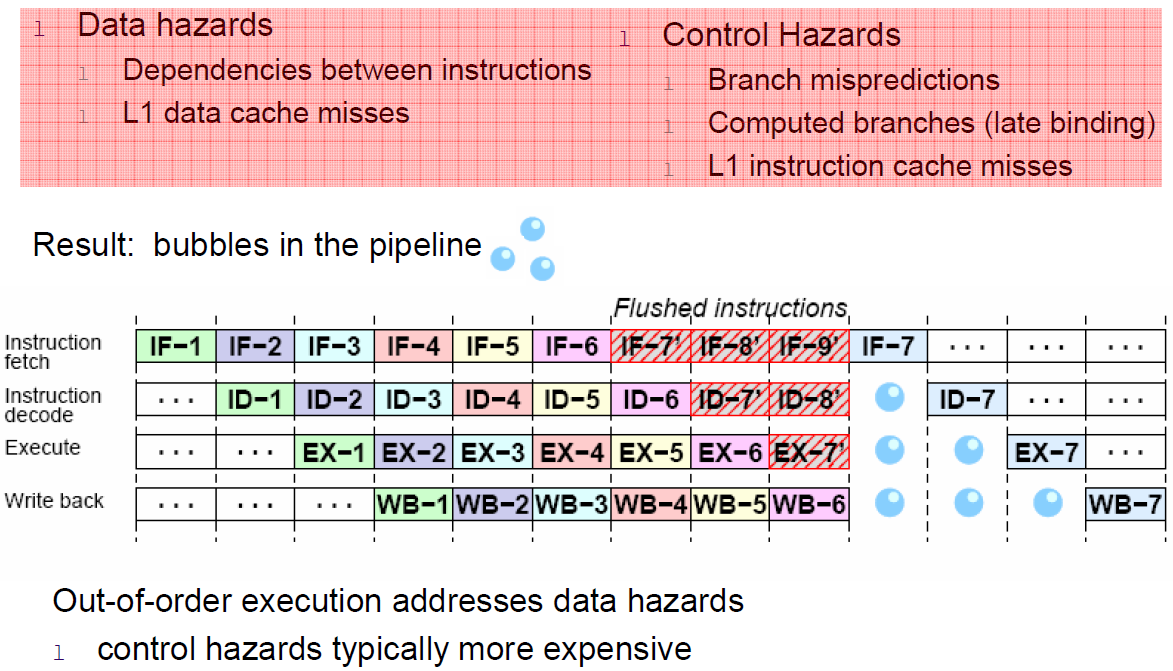
\includegraphics[width=\textwidth,height=0.750\textheight,keepaspectratio]{hazards.png} 
\footnote{\tiny{Изображение взято из \cite{Harizopoulos2009}}}
\end{figure}    
  
\end{frame}

\begin{frame}
\frametitle{Как себя ведет процессор под нагрузкой (итераторами) I}

\begin{figure}[htb]
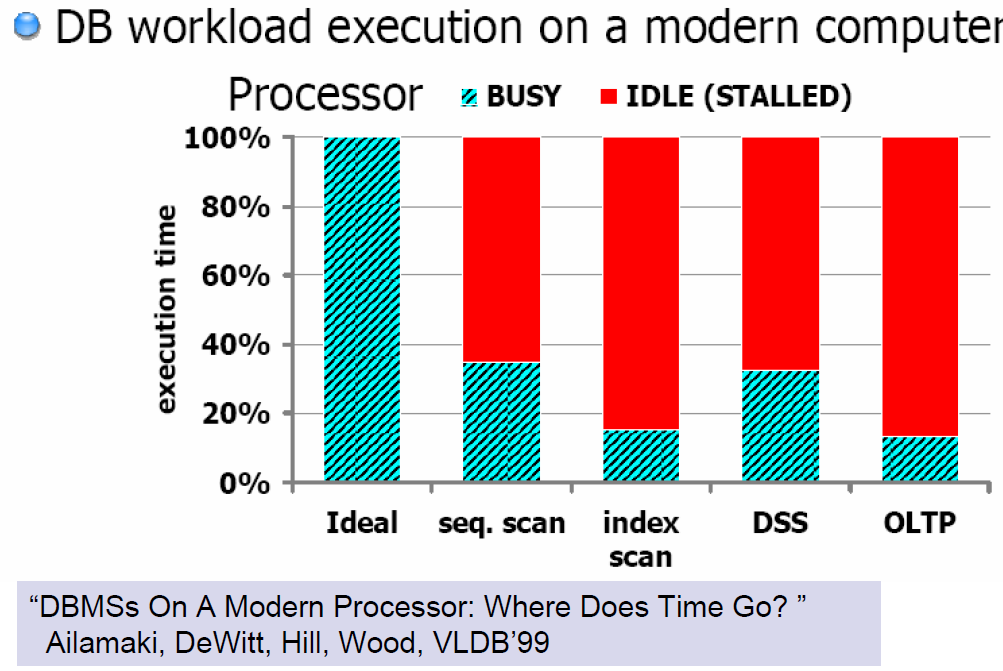
\includegraphics[width=\textwidth,height=0.750\textheight,keepaspectratio]{analysis.png} 
\footnote{\tiny{Изображение взято из \cite{Harizopoulos2009}}}
\end{figure}
  
\end{frame}

\begin{frame}
\frametitle{Как себя ведет процессор под нагрузкой (итераторами) II}

Вкратце из статьи \cite{Boncz2005}:

\begin{itemize}
  \setlength\itemsep{1em}
  \item TPC-H 1GB, Q1 (выборки, агрегация)
  \item Итог:
  \begin{itemize}
    \setlength\itemsep{1em}
    \item C program: 0.2s
    \item MySQL: 26.2s
    \item DBMS ``X'': 28.1s
  \end{itemize}
\end{itemize}
  
\end{frame}

\begin{frame}[fragile]
\frametitle{Как такой (MonetDB) подход помогает?}

Вот так \cite{Boncz2008, Harizopoulos2009}:

\begin{itemize}
  \setlength\itemsep{1em}
  \item ``Хороший''  с точки зрения CPU код:
  \begin{itemize}
    \item Меньше зависимостям по данным;
    \item Меньше зависимостям по управлению;
    \item Можно автоматически генерировать SIMD-код.
  \end{itemize}
  \item Один цикл для целой колонки:
  \begin{itemize}
    \item Отказ от работы на уровне записи;
    \item Массивы позволяют переходить по смещениям;
    \item Лучше ситуация с кешем инструкций.
  \end{itemize}
  
\end{itemize}

\lstset{language=C}

\begin{lstlisting}
{
  for(i=0; i<n; i++)
    res[i] = col[i] - val;
}    
\end{lstlisting}

Итог: Monet около 4s.

\end{frame}

\begin{frame}
\frametitle{Проблемы}

Материализация результата \cite{Boncz2008, Harizopoulos2009}:

\begin{figure}[htb]
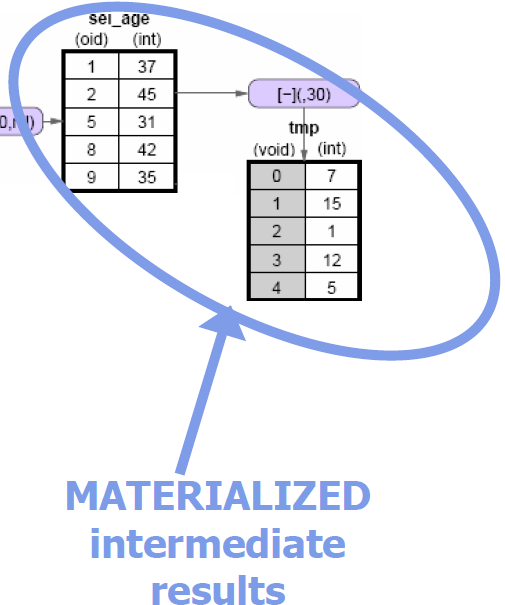
\includegraphics[width=\textwidth,height=0.50\textheight,keepaspectratio]{problems.png} 
\footnote{\tiny{Изображение взято из \cite{Harizopoulos2009}}}
\end{figure}

Памяти просто может не хватить, не будет масштабируемости.
\end{frame}

\begin{frame}
\frametitle{Ниша: исследовательская платформа I}

\begin{figure}[htb]
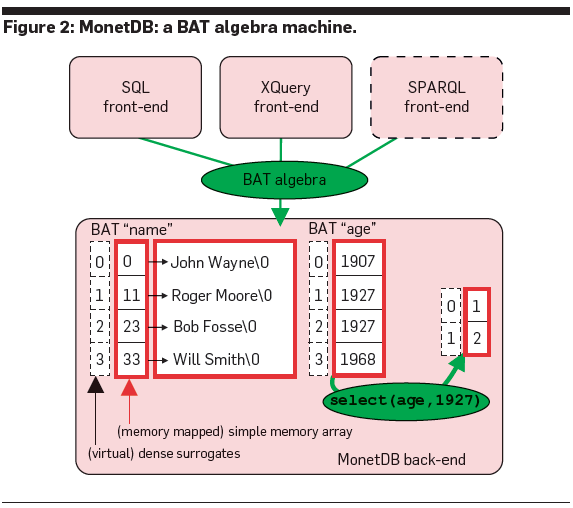
\includegraphics[width=\textwidth,height=0.750\textheight,keepaspectratio]{frontends.png} 
\footnote{\tiny{Изображение взято из \cite{Harizopoulos2009}}}
\end{figure}

\end{frame}

\begin{frame}
\frametitle{Ниша: исследовательская платформа II}

\begin{figure}[htb]
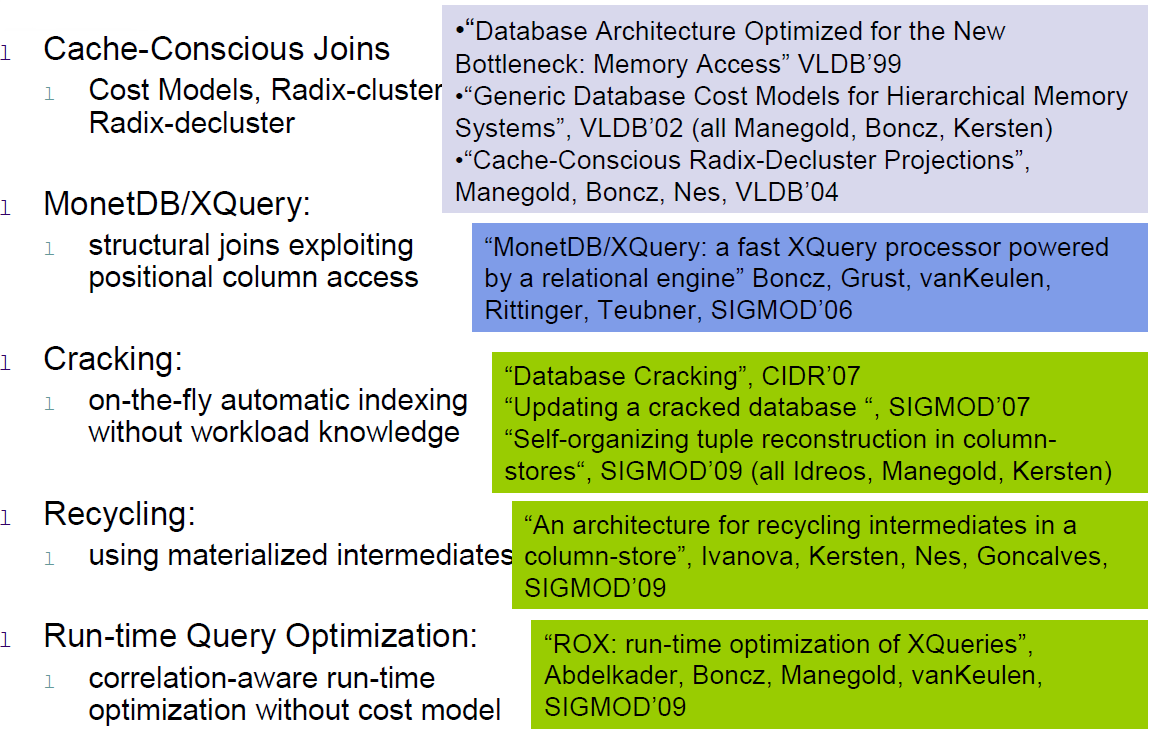
\includegraphics[width=\textwidth,height=0.750\textheight,keepaspectratio]{research.png} 
\footnote{\tiny{Изображение взято из \cite{Boncz2008}}}
\end{figure}

\end{frame}

\begin{frame}
\frametitle{Cache-Conscious Соединение}

Как работает \cite{Shatdal1994}, существующий Grace Hash-Join вариант: 

\begin{itemize}
  \setlength\itemsep{1em}
  \item Оба отношения фрагментируем (по хеш-коду атрибутов соединения) на H кластеров;
  \item Каждый кластер помещается в L2 кеш;
  \item Для каждого кластера ``прикладываем'' элементы соответствующего фрагмента из второго отношения.
\end{itemize}

\end{frame}


\begin{frame}
\frametitle{Проблемы Cache-Conscious Соединения}

Часть с кластеризацией --- проблемная:
\begin{itemize}
  \setlength\itemsep{1em}
  \item Алгоритм имеет один скан и кластеризацию, пишет в H случайных регионов (кластеров), это портит шаблон доступа к памяти;
  \item Если H слишком велико то:
  \begin{itemize}
  	\item записей в TLB может не хватить, будет TLB miss;
  	\item линеек в кеше может не хватить, будет засорение кеша и будут L1, L2 cache miss;  	
  \end{itemize}
  
\end{itemize}

$\longrightarrow$ придумали radix-cluster алгоритм.

\end{frame}

\begin{frame}
\frametitle{Про ``железо'' ``на пальцах'' IX: TLB}

Translation Lookaside Buffer (TLB):
\begin{itemize}
  %\setlength\itemsep{1em}
  \item Тоже ``кеш-память'', встроена в CPU, обеспечивает работу виртуальной памяти;
  \item ``Помнит'' последние трансляции логических в физические адреса (обычно 64-96 штук);
  \item Адресует страницы в оперативной памяти:
  \begin{itemize}
    \item на каждый load/store нужна одна трансляция
    \item нашлась~--- получили адрес сразу же
    \item не нашлась: TLB miss, идем в RAM смотрим в TLB таблицу (тут тоже может быть цепочка из промахов)
  \end{itemize}
  \item При 4KB странице, 64 записи, можно встретить TLB miss при случайном доступе к структурам (хеш-таблицам, например) размером больше чем 256KB.  
\end{itemize}

Сейчас всё сложнее, например на Sandy Bridge отдельные TLB для разных размеров\footnote{\url{https://stackoverflow.com/questions/40649655/how-is-the-size-of-tlb-in-intels-sandy-bridge-cpu-determined}}.

\end{frame}


\begin{frame}
\frametitle{Предложенное решение: radix cluster I}

\begin{figure}[htb]
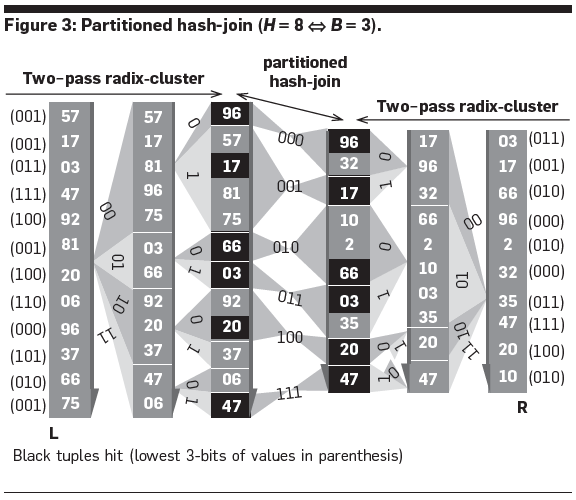
\includegraphics[width=\textwidth,height=0.750\textheight,keepaspectratio]{phjoin.png} 
\footnote{\tiny{Изображение взято из \cite{Boncz2008}}}
\end{figure}

\end{frame}

\begin{frame}
\frametitle{Предложенное решение: radix cluster II}

\begin{itemize}
  \setlength\itemsep{1em}
  \item Перестановка происходит только в рамках блока, лучше паттерн доступа, меньше вероятность промахов;
  \item Обычно хешируют, и работают с хеш-кодами, хотя на рисунке это не показано;
  \item Если колонка начинается с 0 и плотна, можно не хешировать, будет radix-sort.
\end{itemize}
\end{frame}

\begin{frame}
\frametitle{Эксперименты I}

\begin{figure}[htb]
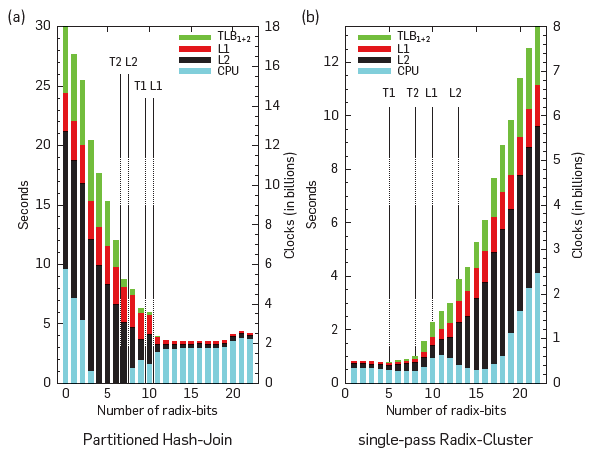
\includegraphics[width=\textwidth,height=0.750\textheight,keepaspectratio]{joinexp1.png} 
\footnote{\tiny{Изображение взято из \cite{Boncz2008}}}
\end{figure}

\end{frame}

\begin{frame}
\frametitle{Эксперименты II}

\begin{figure}[htb]
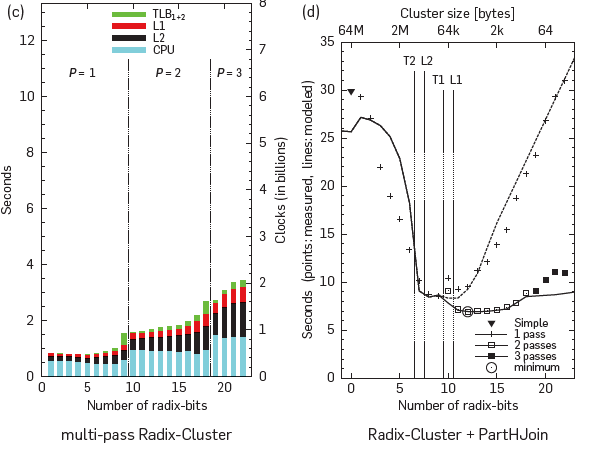
\includegraphics[width=\textwidth,height=0.750\textheight,keepaspectratio]{joinexp2.png} 
\footnote{\tiny{Изображение взято из \cite{Boncz2008}}}
\end{figure}

\end{frame}

\begin{frame}
\frametitle{Database Cracking: идея}

\begin{figure}[htb]
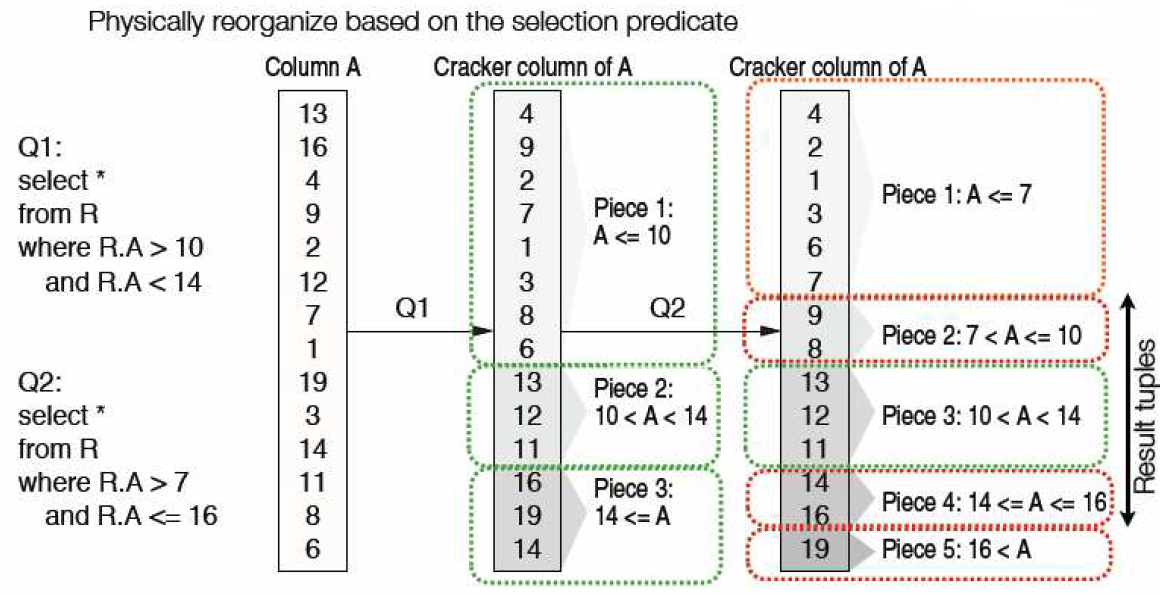
\includegraphics[width=\textwidth,height=0.750\textheight,keepaspectratio]{cracking.png} 
\footnote{\tiny{Изображение взято из \cite{Harizopoulos2009}}}
\end{figure}

\end{frame}

\begin{frame}
\frametitle{Применения Cracking}

\begin{itemize}
  \setlength\itemsep{1em}
  \item Выше было описано как применять к колонкам при запросах на выборку (selection cracking);
  \item Кроме того, можно заменить восстановление записи на cracking (например, вспомните прошлую лекцию, место про соединение и нарушение порядка)~--- sideways cracking.
\end{itemize}
\end{frame}

\begin{frame}
\frametitle{Database Cracking: эксперименты}

\begin{figure}[htb]
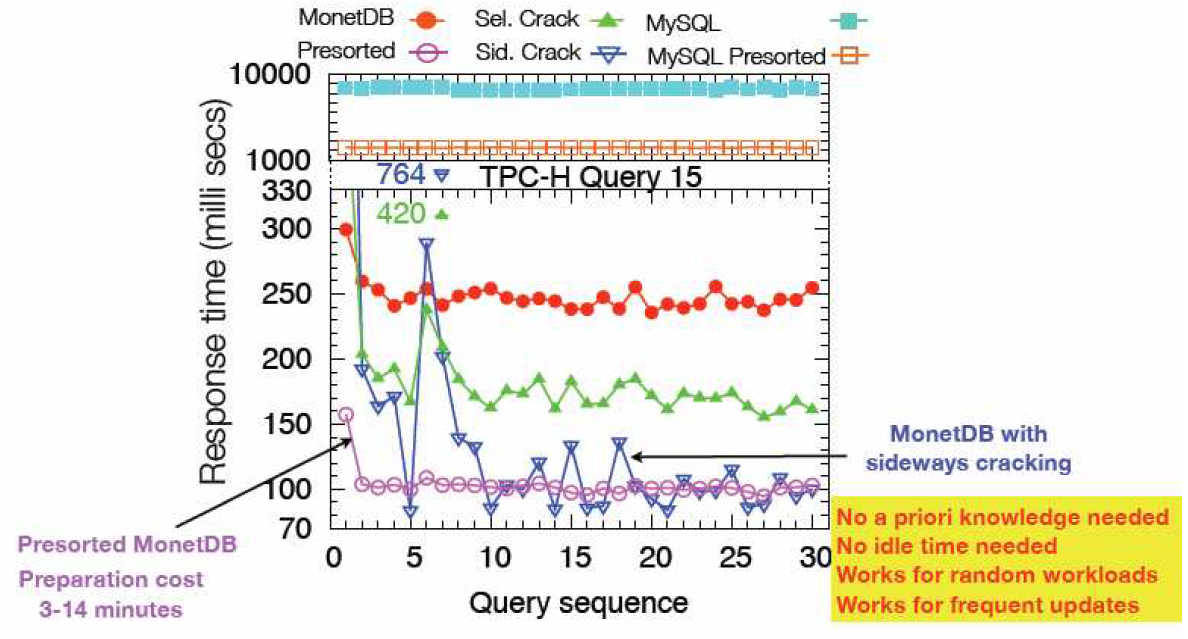
\includegraphics[width=\textwidth,height=0.750\textheight,keepaspectratio]{cracking-experiment.png} 
\footnote{\tiny{Изображение взято из \cite{Harizopoulos2009}}}
\end{figure}

\end{frame}

\begin{frame}
\frametitle{Recycler I: дерево запроса}

\begin{figure}[htb]
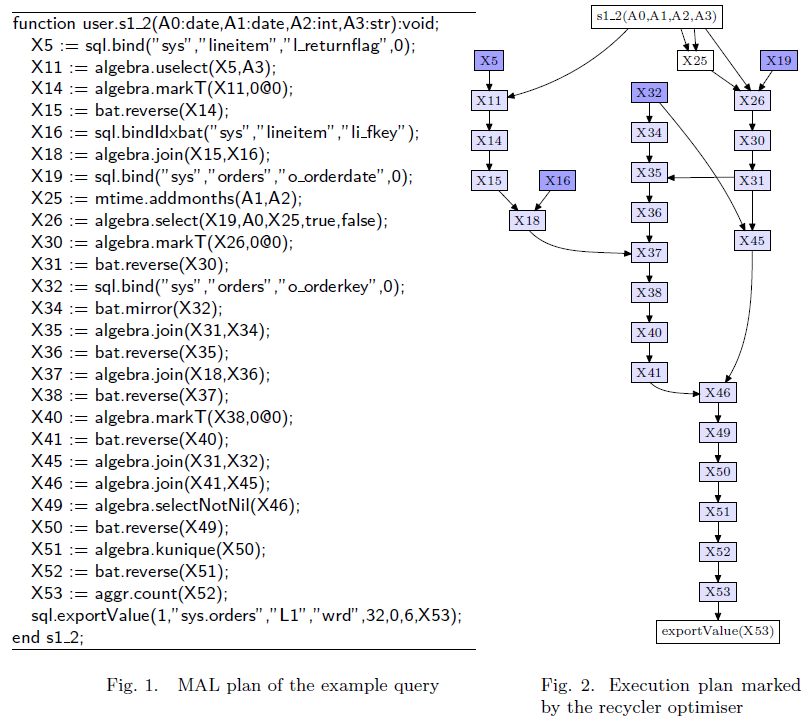
\includegraphics[width=\textwidth,height=0.750\textheight,keepaspectratio]{recycler.png} 
\footnote{\tiny{Изображение взято из \cite{Ivanova2010}}}
\end{figure}

\end{frame}

\begin{frame}
\frametitle{Recycler II: идея}

\begin{itemize}
  \setlength\itemsep{1em}
  \item Полная материализация промежуточных результатов~--- можно переиспользовать некоторые из них:
  \begin{itemize}
    \setlength\itemsep{1em}
    \item Локально: в рамках одного плана + в рамках шаблона;
    \item Глобально: в рамках нескольких параллельно идущих запросов;
  \end{itemize}
  \item Кеш с политикой допуска:
  \begin{itemize}
    \setlength\itemsep{1em}
    \item KEEPALL~--- храним всё;
    \item CREDIT~--- экономические принципы;
  \end{itemize}
  \item ...и с политикой вытеснения:
  \begin{itemize}
    \setlength\itemsep{1em}
    \item LRU;
    \item Benefit policy;
    \item History policy.
  \end{itemize}
  
\end{itemize}
\end{frame}

\begin{frame}
\frametitle{Recycler III: сколько можно сэкономить?}

\begin{figure}[htb]
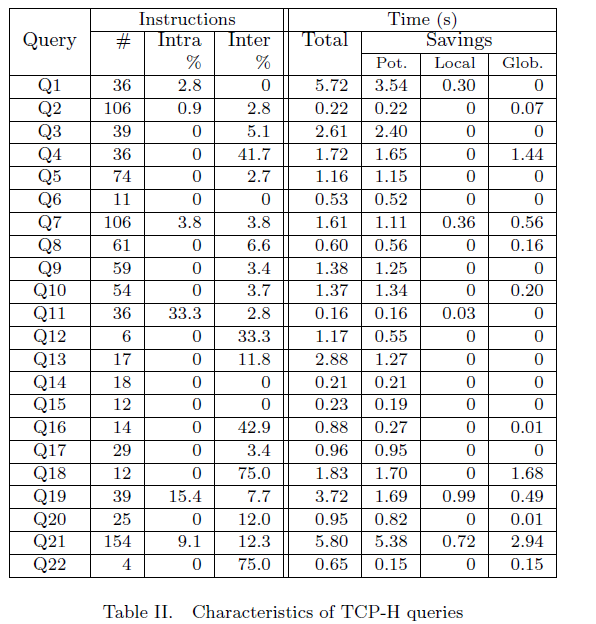
\includegraphics[width=\textwidth,height=0.750\textheight,keepaspectratio]{reccache.png} 
\footnote{\tiny{Изображение взято из \cite{Ivanova2010}}}
\end{figure}

\end{frame}

\begin{frame}
\frametitle{Recycler VI: тест на реальной базе}

\begin{figure}[htb]
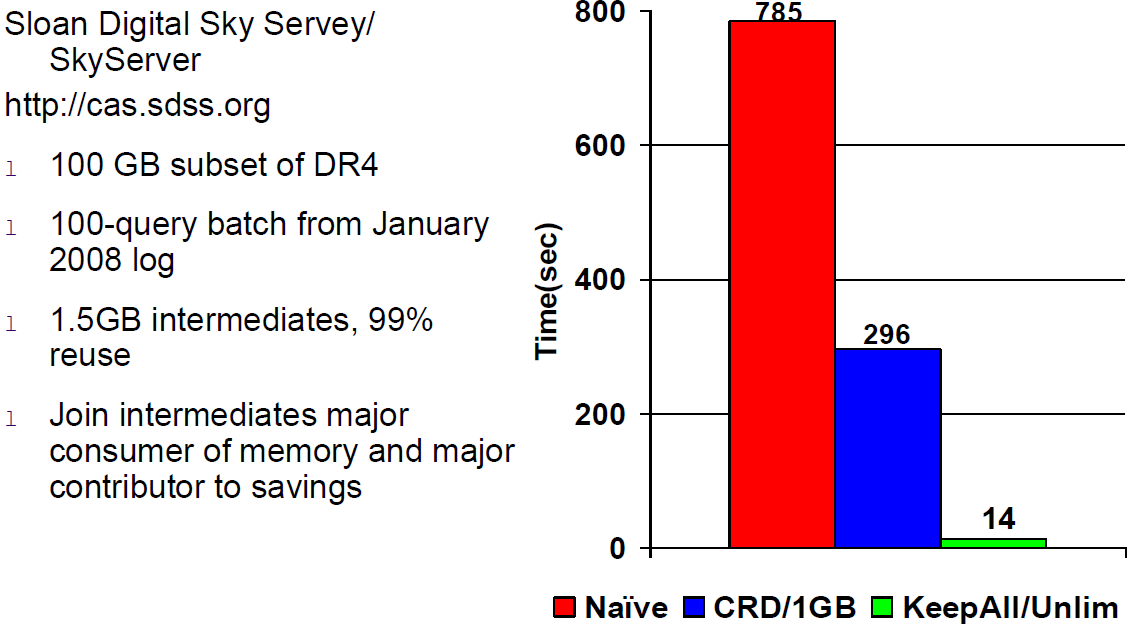
\includegraphics[width=\textwidth,height=0.750\textheight,keepaspectratio]{recres.png} 
\footnote{\tiny{Изображение взято из \cite{Ivanova2010}}}
\end{figure}

\end{frame}

\begin{frame}
\frametitle{Данные на диске в строчных системах}

В двух словах (очень приблизительно):

\begin{itemize}
	\item Данных хранятся на диске;
	\item Считываются и \alert{временно} хранятся в памяти;
	\item Обычно какой-то memory mapping;
	\item Менджер буферов (buffer-manager): считывание, удержание в памяти, модификация данных, сброс на диск;
	\begin{itemize}
		\item pin/unpin;
		\item алгоритм замещения: LRU, Clock algorithm, MRU, ...
	\end{itemize}
	\item ``Нарезка'' на страницы: единицы оперирования менеджера буферов, 4-8 KB;
	\item \alert{Зачем это всё? Управление ресурсами + data sharing.}
\end{itemize}

Кому интересно дальше: \small{\url{https://web.stanford.edu/class/cs346/2015/notes/Lecture_One.pdf}}

Как представлять страницу? Уже обсуждали.

\end{frame}

\begin{frame}
\frametitle{Напоминание: слотированная страница}

\begin{figure}[htb]
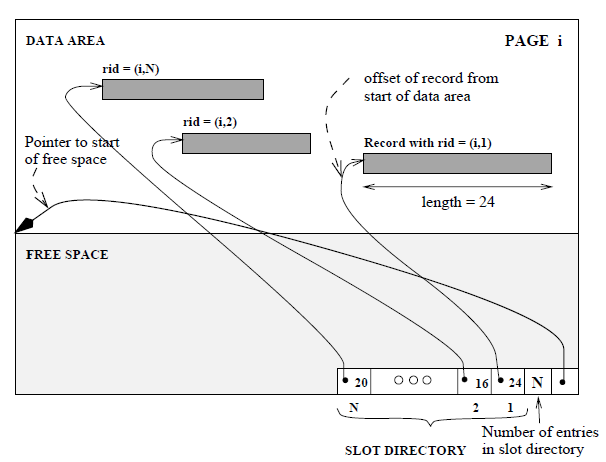
\includegraphics[width=\textwidth,height=0.8\textheight,keepaspectratio]{slotted.png} 
\footnote{\tiny{Изображение взято из \cite{Ramakrishnan2000}}}
\end{figure}

\end{frame}


\begin{frame}
\frametitle{MonetDB/X100 \cite{Boncz2005}}

\begin{itemize}
  \setlength\itemsep{1em}
  \item Избавились от полной материализации и добавили pipelining;
  \item Сделали ``векторизацию'': в кеше массив из ста элементов;
  \begin{itemize}
    \item Все вектора должны помещаться в кеш!
  \end{itemize}
  \item Такие же простые операторы цикла для обработки;
  \item Поздняя материализация + selection vectors: col[sel[i]];  
\end{itemize}

Итог: MonetDB/X100: 0.6s (слайд 16)
\end{frame}

\begin{frame}
\frametitle{MonetDB/X100: архитектура}

\begin{figure}[htb]
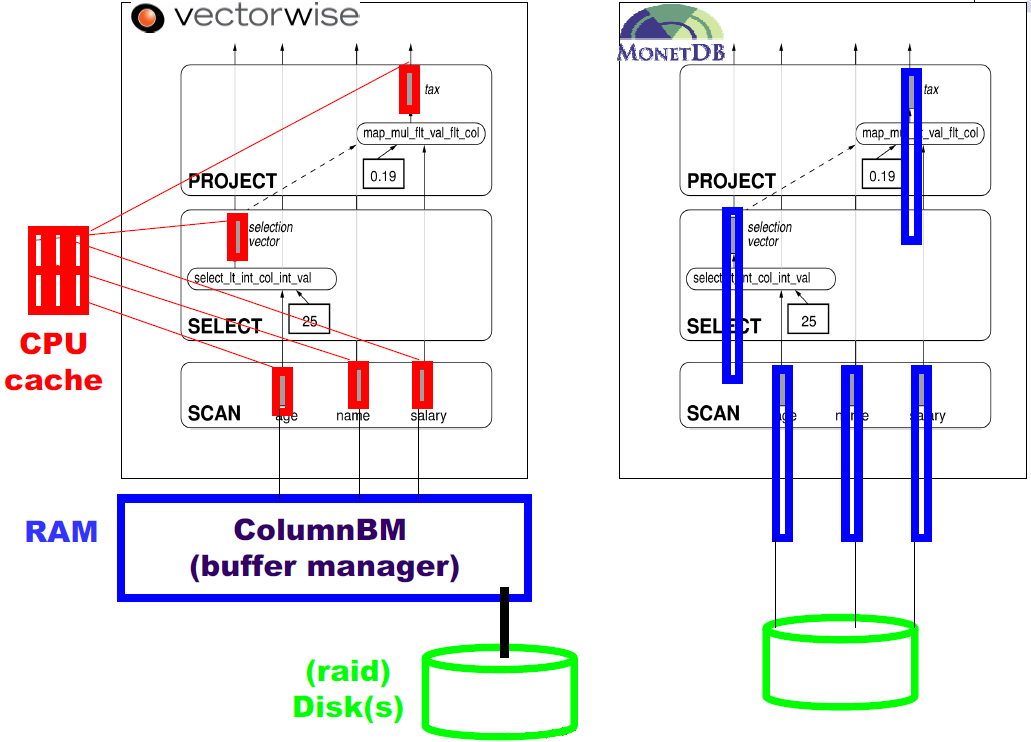
\includegraphics[width=\textwidth,height=0.750\textheight,keepaspectratio]{x100.png} 
\footnote{\tiny{Изображение взято из \cite{Harizopoulos2009}}}
\end{figure}

\end{frame}

\begin{frame}
\frametitle{Пояснение про selection vectors}

\begin{figure}[htb]
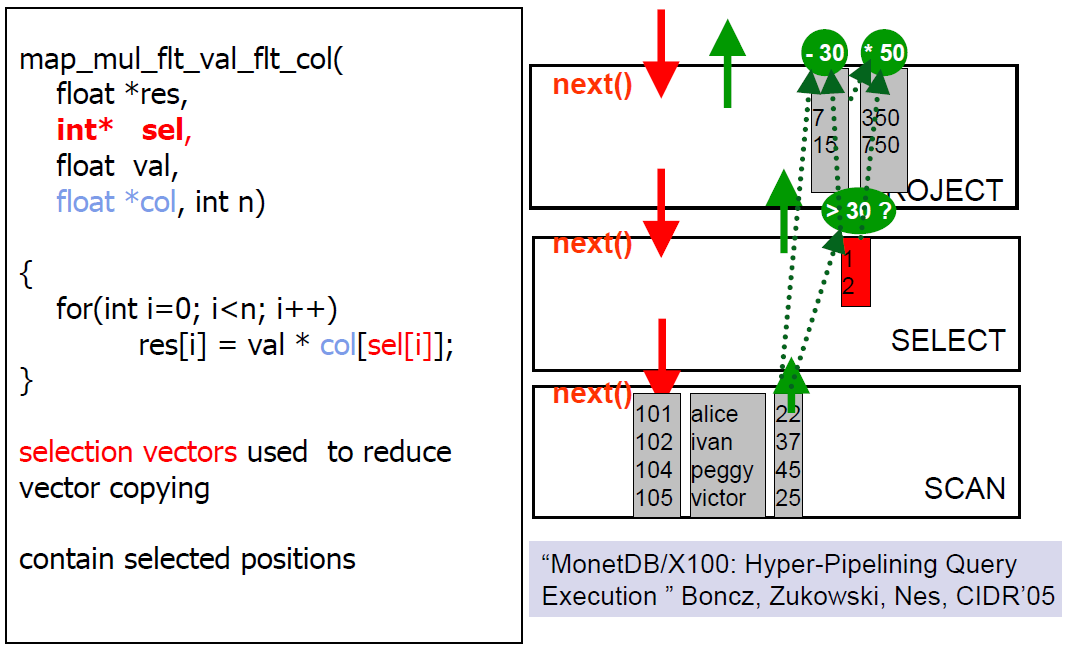
\includegraphics[width=\textwidth,height=0.750\textheight,keepaspectratio]{selectionvecs.png} 
\footnote{\tiny{Изображение взято из \cite{Harizopoulos2009}}}
\end{figure}

\end{frame}

\begin{frame}
\frametitle{MonetDB/X100: размер вектора I}

\begin{figure}[htb]
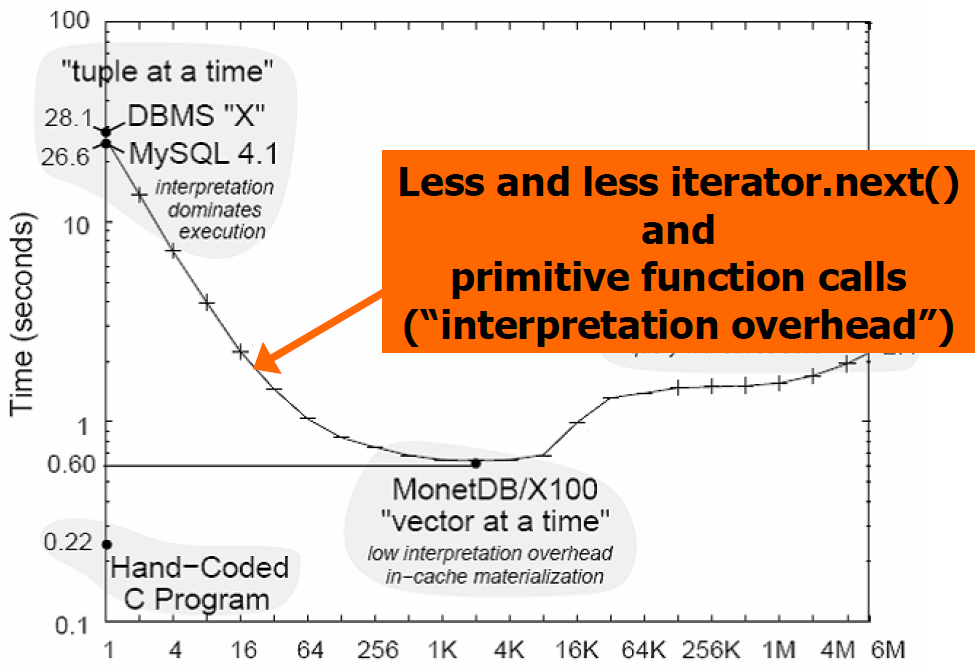
\includegraphics[width=\textwidth,height=0.750\textheight,keepaspectratio]{vecsize1.png} 
\footnote{\tiny{Изображение взято из \cite{Harizopoulos2009}}}
\end{figure}

\end{frame}

\begin{frame}
\frametitle{MonetDB/X100: размер вектора II}

\begin{figure}[htb]
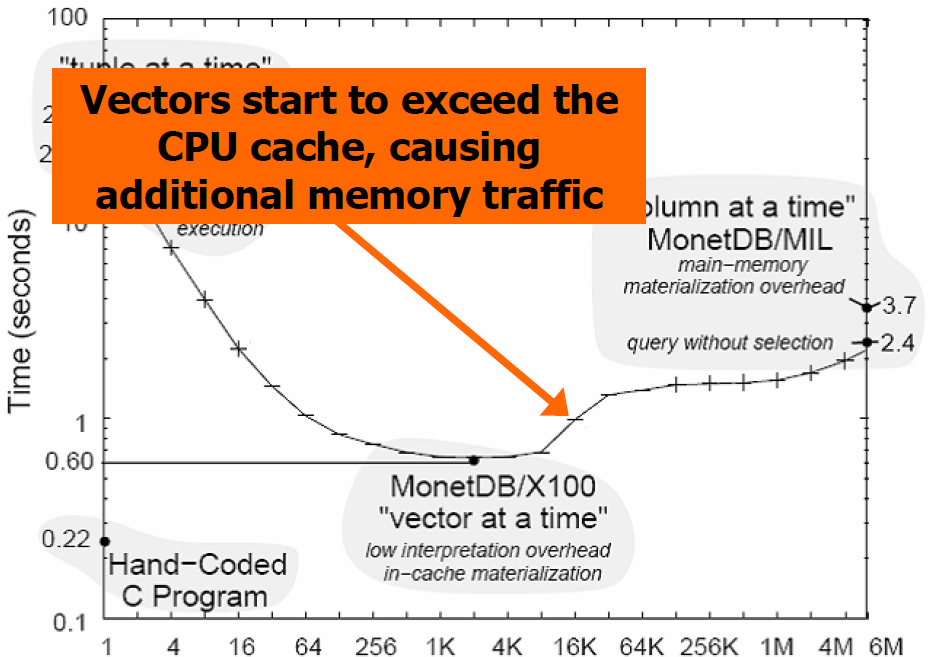
\includegraphics[width=\textwidth,height=0.750\textheight,keepaspectratio]{vecsize2.png} 
\footnote{\tiny{Изображение взято из \cite{Harizopoulos2009}}}
\end{figure}

\end{frame}

\begin{frame}
\frametitle{MonetDB/X100: размер вектора III}

\begin{figure}[htb]
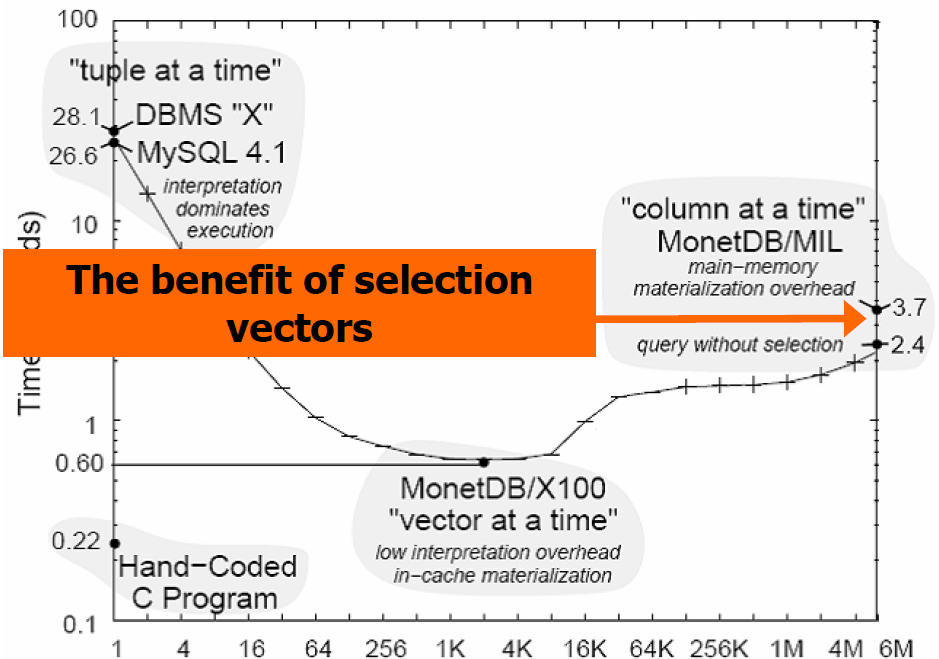
\includegraphics[width=\textwidth,height=0.750\textheight,keepaspectratio]{vecsize3.png} 
\footnote{\tiny{Изображение взято из \cite{Harizopoulos2009}}}
\end{figure}

\end{frame}


\begin{frame}[allowframebreaks]
\frametitle{Ссылки}
\footnotesize{
\begin{thebibliography}{99}

\bibitem[Ivanova et al., 2010] {Ivanova2010} Milena G. Ivanova, Martin L. Kersten, Niels J. Nes, and Romulo A.P. Gonçalves. 2010. An architecture for recycling intermediates in a column-store. ACM Trans. Database Syst. 35, 4, Article 24 (October 2010), 43 pages. DOI=10.1145/1862919.1862921 http://doi.acm.org/10.1145/1862919.1862921 

\bibitem[Shatdal et al., 1994] {Shatdal1994} Ambuj Shatdal, Chander Kant, and Jeffrey F. Naughton. 1994. Cache Conscious Algorithms for Relational Query Processing. In Proceedings of the 20th International Conference on Very Large Data Bases (VLDB '94), Jorge B. Bocca, Matthias Jarke, and Carlo Zaniolo (Eds.). Morgan Kaufmann Publishers Inc., San Francisco, CA, USA, 510--521. 

\bibitem[Boncz et al., 2008] {Boncz2008} Peter A. Boncz, Martin L. Kersten, and Stefan Manegold. 2008. Breaking the memory wall in MonetDB. Commun. ACM 51, 12 (December 2008), 77--85. DOI=http://dx.doi.org/10.1145/1409360.1409380 

\bibitem[Boncz et al., 2005] {Boncz2005} Peter Boncz, Marcin Zukowski, Niels Nes. MonetDB/X100: Hyper-Pipelining Query Execution. CIDR'05.

\bibitem[Boncz and Kersten, 1999]{Boncz1999} Peter A. Boncz and Martin L. Kersten. 1999. MIL primitives for querying a fragmented world. The VLDB Journal 8, 2 (October 1999), 101-119. DOI=http://dx.doi.org/10.1007/s007780050076 

\bibitem[Hennessy and Patterson, 2011] {Hennessy2011}  John L. Hennessy and David A. Patterson. 2011. Computer Architecture, Fifth Edition: A Quantitative Approach (5th ed.). Morgan Kaufmann Publishers Inc., San Francisco, CA, USA. 

\bibitem[Harizopoulos and Ailamaki, 2006] {Harizopoulos2006} Stavros Harizopoulos and Anastassia Ailamaki. 2006. Improving instruction cache performance in OLTP. ACM Trans. Database Syst. 31, 3 (September 2006), 887-920. DOI=http://dx.doi.org/10.1145/1166074.1166079 

%\bibitem[Tsirogiannis et al., 2009] {Tsirogiannis2009}  Dimitris Tsirogiannis, Stavros Harizopoulos, Mehul A. Shah, Janet L. Wiener, and Goetz Graefe. 2009. Query processing techniques for solid state drives. In Proceedings of the 2009 ACM SIGMOD International Conference on Management of data (SIGMOD '09), Carsten Binnig and Benoit Dageville (Eds.). ACM, New York, NY, USA, 59-72. DOI=http://dx.doi.org/10.1145/1559845.1559854 

%\bibitem[Li and Ross, 1999] {Li1999} Zhe Li and Kenneth A. Ross. 1999. Fast joins using join indices. The VLDB Journal 8, 1 (April 1999), 1--24. DOI=http://dx.doi.org/10.1007/s007780050071 

%\bibitem[Star Schema Benchmark Specification, 2009] {SSB} Star Schema Benchmark. Revision 3, June 5, 2009 Pat O'Neil, Betty O'Neil, Xuedong Chen

%\bibitem[Abadi et al., 2008] {Abadi2008} Daniel J. Abadi, Samuel R. Madden, and Nabil Hachem. 2008. Column-stores vs. row-stores: how different are they really?. In Proceedings of the 2008 ACM SIGMOD international conference on Management of data (SIGMOD '08). ACM, New York, NY, USA, 967-980. DOI=http://dx.doi.org/10.1145/1376616.1376712 

%\bibitem[TPC-H Specification, 2011] {TPC-H} TPC BENCHMARK(TM) H (Decision Support) Standard Specification Revision 2.14.2

\bibitem[Abadi et al., 2012] {Abadi2013} Daniel Abadi, Peter Boncz, Stavros Harizopoulos. The Design and Implementation of Modern Column-Oriented Database Systems. Foundations and Trends(R) in Databases Vol. 5, No. 3 (2012) 197--280

\bibitem[Harizopoulos et al., 2009] {Harizopoulos2009} Stavros Harizopoulos, Daniel Abadi, Peter Boncz. Column-Oriented Database Systems. VLDB 2009 Tutorial (slides).

% \bibitem[Чернышев, 2013] {Chernishev2013}	Г. А. Чернышев, <<Организация физического уровня колоночных СУБД>>, Тр. СПИИРАН, 30 (2013), 204--222

% \bibitem[Кузнецов, 2010] {Kuznetsov2010}	 Кузнецов С.Д., <<Год эпохи перемен в технологии баз данных>>, Труды Института системного программирования РАН, 19 (2010), 9--34

%\bibitem[Elnikety, 2009] {Elnikety2009} Distributed DBMS. Sameh Elnikety. Encyclopedia of Database Systems. Ling Liu and M. Tamer {\"O}zsu (eds), p. 896--899. Springer US, 2009. \url{http://dx.doi.org/10.1007/978-0-387-39940-9\_654}

%\bibitem[Kian-Lee Tan, 2009] {Kian-Lee2009} Distributed Database Systems. Kian-Lee Tan. Encyclopedia of Database Systems. Ling Liu and M. Tamer {\"O}zsu (eds), p. 894--896. Springer US, 2009. \url{http://dx.doi.org/10.1007/978-0-387-39940-9_701}

%\bibitem[{\"O}zsu and Valduriez, 2009] {Ozsu2011} {\"O}zsu M.T. and Valduriez P. Principles of Distributed Database Systems, 3rd ed. Prentice-Hall, 2011.

%\bibitem[Kossmann, 2000] {Kossmann2000} Donald Kossmann. 2000. The state of the art in distributed query processing. ACM Comput. Surv. 32, 4 (December 2000), 422--469. DOI=http://dx.doi.org/10.1145/371578.371598 


%\bibitem[Ioannidis, 2003] {Ioannidis2003}  Yannis Ioannidis. 2003. The history of histograms (abridged). In Proceedings of the 29th international conference on Very large data bases - Volume 29 (VLDB '03), Johann Christoph Freytag, Peter C. Lockemann, Serge Abiteboul, Michael J. Carey, Patricia G. Selinger, and Andreas Heuer (Eds.), Vol. 29. VLDB Endowment 19--30. 

%\bibitem[Ioannidis and Poosala, 1995] {Ioannidis1995} Y. Ioannidis and V. Poosala. Histogram Based Solutions to Diverse Database Estimation Problems, IEEE Data Engineering, Vol. 18, No. 3, pp. 10--18, September 1995.

%\bibitem[Poosala et al., 1996] {Poosala1996} Viswanath Poosala, Peter J. Haas, Yannis E. Ioannidis, and Eugene J. Shekita. 1996. Improved histograms for selectivity estimation of range predicates. In Proceedings of the 1996 ACM SIGMOD international conference on Management of data (SIGMOD '96), Jennifer Widom (Ed.). ACM, New York, NY, USA, 294--305. DOI=http://dx.doi.org/10.1145/233269.233342 


%\bibitem[Kooi, 1980] {Kooi1980} Robert Philip Kooi. The Optimization of Queries in Relational Databases. PhD Thesis, Case Western Reserve University (1980).

%\bibitem[Piatetsky-Shapiro and Connel, 1984] {Piatetsky-Shapiro1984} Gregory Piatetsky-Shapiro and Charles Connell. 1984. Accurate estimation of the number of tuples satisfying a condition. In Proceedings of the 1984 ACM SIGMOD international conference on Management of data (SIGMOD '84). ACM, New York, NY, USA, 256--276. DOI=http://dx.doi.org/10.1145/602259.602294 


%\bibitem[Garcia-Molina et al., 2004] {Ulman2004} Гектор Гарсиа-Молина, Джеффри Д. Ульман, Дженнифер Уидом. Системы баз данных. Полный курс.  ISBN 5-8459-0384-Х; 2004 г. 

%\bibitem[Hellerstein et al., 2007] {Hellerstein2007} Joseph M. Hellerstein, Michael Stonebraker, and James Hamilton. Architecture of a Database System. Found. Trends databases 1, 2 (February 2007), 141--259. 

%\bibitem[Neumann, 2009] {Neumann2009} Thomas Neumann. Query Optimization (in Relational Databases). Encyclopedia of Database Systems. Springer US, 2009. 2273--2278.\url{http://dx.doi.org/10.1007/978-0-387-39940-9_293}

%\bibitem[Selinger et al., 1979] {Selinger1979} Selinger P.G., Astrahan M.M., Chamberlin D.D., Lorie R.A., and Price T.G. Access path selection in a relational database management System. In Proc. ACM SIGMOD Int. Conf. on Management of Data, 1979, pp. 23--34.

%\bibitem[Haas et al., 1989] {Haas1989} Haas L.M., Freytag J.C., Lohman G.M., and Pirahesh H. Extensible query processing in starburst. In Proc. ACM SIGMOD Int. Conf. on Management of Data, 1989, pp. 377--388.

%\bibitem[Graefe, 1995] {Graefe1995} Graefe G. The cascades framework for query optimization. Q. Bull. IEEE TC on Data Engineering, 18(3):19--29, 1995.

%\bibitem[Graefe and McKenna, 1993] {Graefe1993} Graefe G. and McKenna W.J. The volcano optimizer generator: Extensibility and efficient search. In Proc. 9th Int. Conf. on Data Engineering, 1993, pp. 209--218.

%\bibitem[Chaudhuri, 1998] {Chaudhuri1998} Chaudhuri S. An overview of query optimization in relational systems. In Proc. 17th ACM SIGACT-SIGMOD-SIGART Symp. Principles of Database Systems, 1998, pp. 34--43.

%\bibitem[Ioannidis, 1996] {Ioannidis1996} Ioannidis Y. Query optimization. In Handbook of Computer Science, A.B. Tucker (ed.). CRC Press, 1996.

%\bibitem[Jarke and Koch, 1984] {Chaudhuri1984} Jarke M. and Koch J. Query optimization in database systems. ACM Comput. Surv., 16(2):111–152, 1984.

%\bibitem[Ioannidis, 1996] {Ioannidis1996} Yannis E. Ioannidis. 1996. Query optimization. ACM Comput. Surv. 28, 1 (March 1996), 121--123. DOI=http://dx.doi.org/10.1145/234313.234367 

%\bibitem[Graefe, 1996] {Graefe1996} Goetz Graefe. 1996. Iterators, schedulers, and distributed-memory parallelism. Softw. Pract. Exper. 26, 4 (April 1996), 427--452. DOI=http://dx.doi.org/10.1002/(SICI)1097-024X(199604)26:4<427::AID-SPE20>3.3.CO;2-8 

%\bibitem[Taniar et al., 2008] {Taniar2008} David Taniar, Clement H. C. Leung, Wenny Rahayu, and Sushant Goel. 2008. High Performance Parallel Database Processing and Grid Databases. Wiley Publishing. 

\bibitem[Ramakrishnan and Gehrke, 2000] {Ramakrishnan2000}  Raghu Ramakrishnan and Johannes Gehrke. 2000. Database Management Systems (2nd ed.). Osborne/McGraw-Hill, Berkeley, CA, USA. 

\end{thebibliography}
}
\end{frame}


\end{document} 